\documentclass[•]{article}

\usepackage{graphicx}


\title{ CSC 447 - Artificial Neural Networks }
\author{Stephanie Athow, Ben Kaiser, Marcus Haberling}
\date{ \today }



\begin{document}
\maketitle

\section{Training results}
\textit{How well does your network train? }

The following results were run on a neural network topology of 25 input nodes, 3 or 4 hidden nodes (dependent on which parameter file was used) and 3 output nodes.

Our network appears to train really well. With 1-2 training sessions, the RMS values are often below 0.12 for both the Black Hills data and the Northwest South Dakota data.

After training the network with the Black Hills data, if the same Black Hills data is run as a test, the accuracy we got was between 94\% and 100\%. However, when the Northwest data was run on a Black Hills trained net, the accuracy was lower. We got between 75\% and 81.25\%. 

\begin{center}
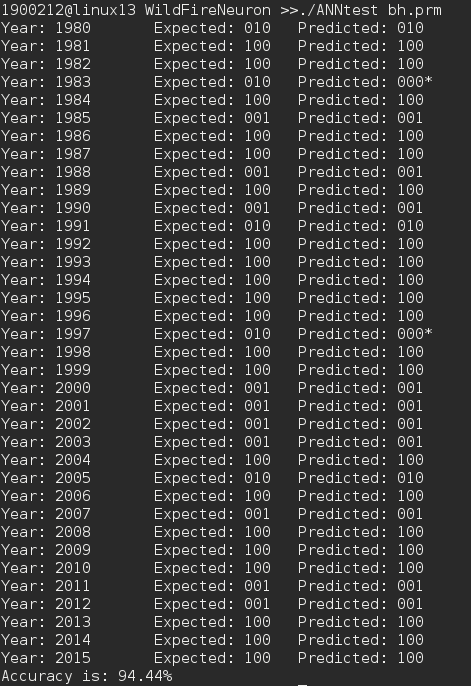
\includegraphics[width=0.5\textwidth]{pictures/Test1BHtrainBHtest.png}
\end{center}

\section{Network Topology}
\textit{What is the impact of network topology (i.e., changing the number of hidden layer nodes) on training? }

\section{Generalization of Data}
\textit{How well does the network generalize from training data to testing data?}

\end{document}